% \documentclass[12pt]{article}
% %\pdfminorversion=4
% \usepackage{geometry}
% \geometry{letterpaper}
% \usepackage{graphicx}
% \usepackage{lscape}
% \usepackage{comment}
% \usepackage{setspace}
% \usepackage{amsmath}
% \usepackage[labelfont=bf,labelsep=period]{caption}
% \renewcommand{\figurename}{Fig.}
% \usepackage{booktabs}
% \usepackage[sectionbib]{chapterbib}
% \usepackage{url}
% %\urlstyle{rm}
% \usepackage{titlesec}
% \usepackage[usenames,dvipsnames]{xcolor}
% \DeclareTextCommandDefault{\nobreakspace}{\leavevmode\nobreak\ }
%
% \usepackage[round]{natbib}
% \bibpunct{(}{)}{;}{a}{}{;}

%\hyphenation{meta-pop-ulation meta-pop-ulations sub-pop-ulations sub-pop-ulation}

%\newcommand{\CV}{\mathrm{CV}}

%\title{Supporting Information for\\Ecological prophets:\\Quantifying metapopulation portfolio effects\\Methods in Ecology and Evolution}

%\author{Sean C. Anderson$^{1*}$ \and Andrew B. Cooper$^2$ \and Nicholas K. Dulvy$^1$}

%\date{}

%\textheight 20.5cm

%\setcounter{secnumdepth}{-2}

%\newcommand{\tilmanPE}{mean-variance PE}
%\newcommand{\schindlerPE}{average-CV PE}
%\newcommand{\zvalue}{$z$-value}
%
%\newcommand{\drivers}{Fig.~\ref{fig:PE-drivers}}
%\newcommand{\driverszcol}{Fig.~\ref{fig:PE-drivers-z-colour}}
%\newcommand{\driverscor}{Fig.~\ref{fig:factors-cor}}


%\newlabel{fig:didactic}{{1}{25}}
%\newlabel{fig:lines}{{2}{26}}
%\newlabel{fig:meta}{{3}{27}}
%\newlabel{fig:detrend}{{4}{28}}
%\newlabel{fig:paramspace}{{5}{29}}
%\newlabel{fig:recommendations}{{6}{30}}

%\begin{document}

%\maketitle

% \noindent
%   \textsuperscript{1}Earth to Ocean Research Group, Department of Biological
%   Sciences, Simon Fraser University, Burnaby BC, V5A 1S6, Canada
%
% \noindent
% 	\textsuperscript{2}School of Resource and Environmental Management, Simon
%   Fraser University, Burnaby, BC, V5A 1S6, Canada
%
% \noindent
% 	\textsuperscript{*}Corresponding author: sean\_anderson@sfu.ca
%
%\newpage

%\begin{spacing}{1.2}
%\section{Ecological prophets: Quantifying metapopulation portfolio effects}
%\noindent
%Sean C. Anderson, Andrew B. Cooper, Nicholas K.  Dulvy

%\section*{Supporting Information}

\chapter{Supporting materials}{Supporting materials for Ecological prophets: quantifying metapopulation portfolio effects}

\section{\texttt{R} package to estimate metapopulation portfolio effects}

In an \texttt{R} console, the \texttt{ecofolio} package can be installed either
from the included source package (\texttt{.tar.gz} file)
%, from the Mac or
%Windows binary packages (\texttt{.tgz} or \texttt{.zip}, respectively)
or via the web (instructions below). First, install dependencies if needed:

\begin{verbatim}
install.packages(c("plyr", "reshape", "MuMIn", "robustbase"))
\end{verbatim}

\noindent
Then, to install the included package:

%install.packages("ecofolio_0.1.tar.gz", type = "source")

\begin{verbatim}
install.packages("mee312093-sup-0001-Sourcepackage.tar.gz", type = "source")
\end{verbatim}

%install.packages("ecofolio_0.1.tgz") # Mac binary
%install.packages("ecofolio_0.1.zip") # Windows binary

\noindent
or to install the current version from the web:

\begin{verbatim}
install.packages("devtools") # if needed
devtools::install_github("ecofolio", username = "seananderson")
\end{verbatim}

\noindent
Current code and install details are available at\\ \url{https://github.com/seananderson/ecofolio}
\clearpage

%Install details are available at:
%\url{https://github.com/seananderson/ecofolio}

\noindent
You can load the package, read the vignette, and access the help pages with:

\begin{verbatim}
library(ecofolio)
vignette("ecofolio")
help(package = "ecofolio")
\end{verbatim}

\section{Data sources for the empirical portfolio effect analysis}
We sought to include as many metapopulation time series from as diverse
taxonomic groups as possible. However, due to availability, the included data
primarily represent metapopulations in North America (salmon), the United
Kingdom (moths), and Australia (reef fishes) (Figure~\ref{fig:map}). We show a
summary of the data included in our analysis of empirical ecological systems
in Table S1 and the time series in Figure~\ref{fig:ts}.

\subsection{Salmon}
We obtained salmon data from a variety of sources, in particular
\citet{dorner2008}. Most of the salmon populations are from the northwest
coast of North America, but also: Kola Peninsula, Russia
\citep{jensen1999}, southern New England \citep{kocik2006}, and
Central Valley, California \citep{carlson2011} (Figure~\ref{fig:map}). All
data represent annual estimated returns --- fisheries catch plus escapement to
the spawning grounds. We divided pink salmon annual estimated returns into odd-
and even-year time series due to their strongly distinct runs that do not
interbreed \citep{quinn2005}. To maintain consistency with previous PE
analyses involving sockeye salmon \citep{schindler2010} and analyses of
time series of these data \citep{dorner2008}, and due to the less distinct
separate runs \citep{quinn2005}, we did not divide the sockeye salmon into
separate runs.

Subsets of these salmon data have been used in numerous analyses relating
diversity with stability. A particular feature of the salmon literature is a
focus on the role of ``biocomplexity'' --- a diversity of life-histories and
local adaptations to the environment --- in producing stability
\citep{hilborn2003} and recent papers have focussed on measuring the
portfolio effects we investigate in this paper \citep{schindler2010,
  carlson2011}. In studying the mechanisms behind subpopulation
asynchrony, and hence portfolio effects, studies of Pacific salmon have
generally focussed on drivers that fall into two categories: (1) landscape
filtering of the environment so that different subpopulations experience
different environmental forces (e.g.\ local topology affecting stream flow)
\citep[e.g.][]{schindler2008}, and (2) biologically-based response
diversity to the environment (e.g.\ genetically-based variation in thermal
tolerances) \citep[e.g.][]{eliason2011}. These patterns of asynchrony can
play out not just at the decadal scale but also over centuries
\citep{rogers2013}.

\subsection{Moths}
We obtained moth abundance time series from the Rothamsted Insect Survey
(RIS). L. R. Taylor started the trap network that forms the RIS in the early
1960s; the RIS is now one of the longest-running and largest-scale insect
surveys in the world \citep{conrad2004}. Details on the survey are
available in \citet{conrad2004} and \citet{taylor1986}. The RIS
captures moths by light traps \citep{williams1948} placed 1--2 m above
ground; these traps catch small but reliable samples of moth populations
\citep{williams1948, taylor1974, conrad2004}. Although
different species may show different responses to the traps
\citep{muirhead-thomson1991, woiwod1992}, we compare across sites
within the same species so this should not affect our results.

Our moth data spanned from 1999--2010 for 13 species (Table~S1) and 28 sites
(Table~\ref{tab:ris-meta}). We included only moths with single broods per year
(univoltine moths) and single annual flight episodes since we were aggregating
the data annually to maintain consistency with data from other taxonomic
groups that were available. We removed site-species combinations where there
were eight or more years with zero moths caught in traps to avoid sites where
a given species was exceptionally rare and not likely to be consistently
censused. This removed 97 subpopulations leaving 280. Further culling of
populations according to the criteria in the Methods section left us with 268
subpopulations. All the species included are common within Great Britain,
although some have undergone declines in abundance since the RIS began
\citep{conrad2004}.

Earlier versions of these moth data featured heavily in the work of
Taylor and colleagues on the property now known as Taylor's power law
\citep{taylor1977, taylor1980, perry1981}. This early work
focussed on behavioural properties that might regulate the stability and
variance of moth populations \citep{taylor1980}. Work has continued with
these datasets and studies have shown a number of mechanisms generating
stability. For example, authors have shown spatial asynchrony
\citep{gaston1988}, polyphagy (eating different kinds of food)
\citep{redfearn1988}, and density dependence to act as stabilizing forces
\citep{hanski1993}.

\subsection{Reef fishes}

We obtained reef visual census fish counts within the Greater Barrier Reef
(GBR) from the Australian Institute of Marine Science's (AIMS) Long-term
Monitoring Program (LTMP) \citep{sweatman2008}. The AIMS survey data used
here are from fixed transects at selected sites across 46 reefs from
1994--2010 (Table~\ref{tab:grb-meta}). Details of the sampling design are
available from \citet{halford1994}. Briefly, AIMS surveys reef fish
annually within six sectors of the GBR. AIMS identifies inner-, \mbox{mid-,}
and outer-shelf positions and three reefs within each shelf position. Within
each reef, AIMS chooses three sites of the same habitat and establishes five
permanent 50m transects at 6--9m depth 10m apart and parallel to the reef
crest. Divers count damselfishes (Pomacentrids) on 1m-wide transects and all
other families on 5m-wide transects. AIMS only censuses fish one year or older
since recruitment can be highly spatially and temporally variable. AIMS
conducts annual standardization exercises to avoid temporal bias in counts
within and across divers \citep{halford1994}.

A number of recent studies have used these reef-fish data to
investigate stability-diversity relationships, often focusing on functional
diversity or reef size and isolation. For example, \citet{thibaut2012}
found strong asynchrony of response to the environment between three functional
groups of herbivorous reef fishes, which lead to greater stability. Another
benefit to this functional diversity may be increased disease resistance
\citep{raymundo2009}, presumably enhancing stability. Independent of
functional roles, \citet{mellin2010} found that small, isolated reefs have
higher population variability and therefore higher probability of local
extinction.

\section{Diagnosing the ecological properties of empirical portfolio effects}

We overlaid the empirical PEs in their respective theoretical parameter space
to investigate the ecological properties of real-world metapopulations
(subpopulation correlation, mean-variance scaling, subpopulation number
richness, and evenness). Specifically, we matched the empirical
linear-regression z values and the number of subpopulations with their
theoretical counterparts.

To present our results graphically in Figure~\ref{fig:paramspace}, we categorized
the mean correlation of the empirical subpopulations ($\bar{\rho}$) into bins of
$0 \le \bar{\rho} < 0.25$, $0.25 \le \bar{\rho} < 0.5$, and $0.50 \le \bar{\rho}
< 75$ and matched these with the theoretical PE estimated at the midpoints of
these bins (i.e.\ 0.125, 0.375, and 0.625).  We matched the disparity in
subpopulation size by: (1) calculating the CV of the log of the subpopulation
time series' means, $\CV(\log\mu)$; (2) categorizing the empirical
metapopulations into bins of $0 \le \CV(\log\mu) < 0.3$, $0.3 \le \CV(\log\mu) <
0.6$, and $0.6 \le \CV(\log\mu) < 0.9$; (3) estimating the theoretical PE using
evenly-spaced values from a log-normal distribution with a mean of two and
standard deviation of the midpoints of these bins (i.e.\ 0.15, 0.45, and 0.75).
Here and in Figure~\ref{fig:lines}, we derived these evenly-spaced values as
follows.
We drew subpopulation ($i$) quantiles $q_i$ from the evenly-spaced sequence:
$a_1, a_2, \ldots, a_n$, where $a_1 = 1/(n+1)$ and $a_n = 1-(1/(n+1))$. We then
calculated the subpopulation means at each $q_i$ from a log-normal distribution
with log-mean of two and a log-standard deviation of the ``unevenness value''
times the log-mean.

\bibliographystyle{apalike}
\bibliography{/Users/seananderson/Dropbox/tex/jshort,/Users/seananderson/Dropbox/tex/ref3}
\clearpage

%\renewcommand{\thetable}{A\arabic{table}}
%\setcounter{table}{0}

%\renewcommand{\thefigure}{A\arabic{figure}}
%\renewcommand{\figurename}{Figure}
%\setcounter{figure}{0}

\section{Supporting Tables and Figures}

\begin{landscape}


  % latex table generated in R 2.15.0 by xtable 1.7-0 package
% Tue Sep 18 15:07:29 2012
\begin{table}[ht]
\begin{center}
\caption{Metapopulations used in the empirical PE analyses. ID column numbers correspond to ID numbers in the figures.}
\label{tab:datasources}
{\tiny
\begin{tabular}{rlllrrl}
  \toprule
ID & Species & Common & Location & Subpopulations & Years & Reference \\ 
  \midrule
  1 & \textit{Oncorhynchus kisutch} & Coho salmon & Broughton archipelago, BC, Canada &   6 &  16 & \citep{krkosek2011} \\ 
    2 & \textit{Oncorhynchus gorbuscha} & Pink salmon, odd years & Puget Sound, WA, United States &   4 &  19 & \citep{dorner2008} \\ 
    3 & \textit{Oncorhynchus nerka} & Sockeye salmon & Bristol Bay, AK, United States &   8 &  43 & \citep{west2006} \\ 
    4 & \textit{Oncorhynchus nerka} & Sockeye salmon & Kodiak, AK, United States &   4 &  24 & \citep{dorner2008} \\ 
    5 & \textit{Oncorhynchus gorbuscha} & Pink salmon, odd years & Broughton archipelago, BC, Canada &   7 &  19 & \citep{krkosek2011} \\ 
    6 & \textit{Oncorhynchus nerka} & Sockeye salmon & Fraser River, BC, Canada &  16 &  44 & \citep{dorner2008} \\ 
    7 & \textit{Oncorhynchus gorbuscha} & Pink salmon, odd years & Kodiak, AK, United States &   5 &   8 & \citep{dorner2008} \\ 
    8 & \textit{Oncorhynchus gorbuscha} & Pink salmon, even years & Chignik, AK, United States &   5 &  16 & \citep{dorner2008} \\ 
    9 & \textit{Oncorhynchus nerka} & Sockeye salmon & Upper Cook Inlet, AK, United States &   4 &  29 & \citep{fair2011} \\ 
   10 & \textit{Oncorhynchus gorbuscha} & Pink salmon, even years & Broughton archipelago, BC, Canada &   7 &  19 & \citep{krkosek2011} \\ 
   11 & \textit{Salmo salar} & Atlantic salmon & Kola Peninsula, Russia &   4 &  15 & \citep{jensen1999} \\ 
   12 & \textit{Oncorhynchus keta} & Chum salmon & Puget Sound, WA, United States &   7 &  26 & \citep{dorner2008} \\ 
   13 & \textit{Oncorhynchus tshawytscha} & Chinook salmon & Columbia Estuary, OR/WA, United States &   9 &  23 & \citep{streamnet2011} \\ 
   14 & \textit{Oncorhynchus tshawytscha} & Chinook salmon & Elochoman River, WA, United States &   5 &  27 & \citep{streamnet2011} \\ 
   15 & \textit{Oncorhynchus keta} & Chum salmon & Arctic, Yukon, Kuskokwim, US and Canada &   5 &  18 & \citep{dorner2008} \\ 
   16 & \textit{Oncorhynchus gorbuscha} & Pink salmon, odd years & Chignik, AK, United States &   5 &  15 & \citep{dorner2008} \\ 
   17 & \textit{Oncorhynchus gorbuscha} & Pink salmon, even years & Kodiak, AK, United States &   5 &   9 & \citep{dorner2008} \\ 
   18 & \textit{Salmo salar} & Atlantic salmon & Southern New England, United States &   6 &  39 & \citep{kocik2006} \\ 
   19 & \textit{Oncorhynchus tshawytscha} & Chinook salmon & Central Valley, California &   9 &  54 & \citep{carlson2011} \\ 
   20 & \textit{Oncorhynchus keta} & Chum salmon & Alaska Peninsula, AK, United States &   4 &  32 & \citep{dorner2008} \\ 
   21 & \textit{Abraxas grossulariata} & The magpie moth & UK &  15 &  12 & \citep{conrad2004} \\ 
   22 & \textit{Orthosia cerasi} & Common quaker moth & UK &  27 &  12 & \citep{conrad2004} \\ 
   23 & \textit{Hemithea aestivaria} & Common emerald moth & UK &  16 &  12 & \citep{conrad2004} \\ 
   24 & \textit{Xestia xanthographa} & Square-spot rustic moth & UK &  28 &  12 & \citep{conrad2004} \\ 
   25 & \textit{Petrophora chlorosata} & Brown silver-lines moth & UK &  18 &  12 & \citep{conrad2004} \\ 
   26 & \textit{Erannis defoliaria} & Mottled umber moth & UK &  19 &  12 & \citep{conrad2004} \\ 
   27 & \textit{Diarsia mendica} & Ingrailed clay moth & UK &  24 &  12 & \citep{conrad2004} \\ 
   28 & \textit{Agrochola (Leptologia) macilenta} & Yellow-line quaker moth & UK &  23 &  12 & \citep{conrad2004} \\ 
   29 & \textit{Pharmacis lupulina} & Common swift moth & UK &  16 &  12 & \citep{conrad2004} \\ 
   30 & \textit{Poecilocampa populi} & December moth & UK &  25 &  12 & \citep{conrad2004} \\ 
   31 & \textit{Eilema lurideola} & Common footman moth & UK &  20 &  12 & \citep{conrad2004} \\ 
   32 & \textit{Agrotis exclamationis} & Heart and dart moth & UK &  23 &  12 & \citep{conrad2004} \\ 
   33 & \textit{Colotois pennaria} & Feathered thorn moth & UK &  26 &  12 & \citep{conrad2004} \\ 
   34 & \textit{Scarus psittacus} & \textit{Scarus psittacus} & GBR, Australia &  37 &  14 & \citep{sweatman2008} \\ 
   35 & \textit{Pomacentrus moluccensis} & \textit{Pomacentrus moluccensis} & GBR, Australia &  35 &  14 & \citep{sweatman2008} \\ 
   36 & \textit{Acanthochromis polyacanthus} & \textit{Acanthochromis polyacanthus} & GBR, Australia &  40 &  14 & \citep{sweatman2008} \\ 
   37 & \textit{Neopomacentrus azysron} & \textit{Neopomacentrus azysron} & GBR, Australia &  39 &  14 & \citep{sweatman2008} \\ 
   38 & \textit{Chlorurus sordidus} & \textit{Chlorurus sordidus} & GBR, Australia &  37 &  14 & \citep{sweatman2008} \\ 
   39 & \textit{Ctenochaetus spp} & \textit{Ctenochaetus spp} & GBR, Australia &  36 &  14 & \citep{sweatman2008} \\ 
   40 & \textit{Pomacentrus lepidogenys} & \textit{Pomacentrus lepidogenys} & GBR, Australia &  39 &  14 & \citep{sweatman2008} \\ 
   41 & \textit{Plectropomus leopardus} & \textit{Plectropomus leopardus} & GBR, Australia &  37 &  14 & \citep{sweatman2008} \\ 
   42 & \textit{Scarus chameleon} & \textit{Scarus chameleon} & GBR, Australia &  37 &  14 & \citep{sweatman2008} \\ 
   43 & \textit{Chlorurus microrhinos} & \textit{Chlorurus microrhinos} & GBR, Australia &  37 &  14 & \citep{sweatman2008} \\ 
   44 & \textit{Scarus frenatus} & \textit{Scarus frenatus} & GBR, Australia &  36 &  14 & \citep{sweatman2008} \\ 
   45 & \textit{Hemigymnus melapterus} & \textit{Hemigymnus melapterus} & GBR, Australia &  37 &  14 & \citep{sweatman2008} \\ 
   46 & \textit{Hemigymnus fasciatus} & \textit{Hemigymnus fasciatus} & GBR, Australia &  37 &  14 & \citep{sweatman2008} \\ 
   47 & \textit{Scarus niger} & \textit{Scarus niger} & GBR, Australia &  37 &  14 & \citep{sweatman2008} \\ 
   48 & \textit{Epibulus insidiator} & \textit{Epibulus insidiator} & GBR, Australia &  37 &  14 & \citep{sweatman2008} \\ 
   49 & \textit{Chaetodon plebeius} & \textit{Chaetodon plebeius} & GBR, Australia &  35 &  14 & \citep{sweatman2008} \\ 
   50 & \textit{Gomphosus varius} & \textit{Gomphosus varius} & GBR, Australia &  36 &  14 & \citep{sweatman2008} \\ 
   51 & \textit{Chaetodon trifasciatus} & \textit{Chaetodon trifasciatus} & GBR, Australia &  36 &  14 & \citep{sweatman2008} \\ 
   \bottomrule
\end{tabular}
}
\end{center}
\end{table}

\end{landscape}
\clearpage

% latex table generated in R 2.15.0 by xtable 1.7-0 package
% Tue Sep 18 15:07:31 2012
\begin{table}[ht]
\begin{center}
\caption{Moth sites used from the Rothamsted Insect Survey database. Sites are ordered from north to south. County refers to the British County. ``Number of spp.''\ refers to the number of moth species remaining that matched our inclusion criteria.}
\label{tab:ris-meta}
{\footnotesize
\begin{tabular}{llrrrr}
  \toprule
Site name & County & Northing & Easting & Altitude (m) & Number of spp. \\ 
  \midrule
Starcross & South Devon & 821 & 2972 & 9 & 12 \\ 
  Denny Lodge & South Hampshire & 1056 & 4333 & 30 & 10 \\ 
  Bentley Wood & South Wiltshire & 1324 & 4253 & 130 & 12 \\ 
  Winkworth & Surrey & 1412 & 4991 & 130 & 12 \\ 
  Alice Holt & North Hampshire & 1428 & 4803 & 122 & 12 \\ 
  Perry Wood & East Kent & 1565 & 6040 & 80 & 13 \\ 
  Wisley II & Surrey & 1579 & 5065 & 40 & 10 \\ 
  Westonbirt & West Gloucestershire & 1898 & 3847 & 46 & 13 \\ 
  Geescroft I & Hertfordshire & 2128 & 5132 & 130 & 12 \\ 
  Allotments & Hertfordshire & 2134 & 5134 & 130 & 7 \\ 
  Barnfield & Hertfordshire & 2135 & 5132 & 130 & 10 \\ 
  Hereford & Herefordshire & 2476 & 3564 & 91 & 10 \\ 
  Cockayne Hatley & Bedfordshire & 2494 & 5253 & 76 & 11 \\ 
  Llysdinam & Breconshire  & 2586 & 3009 & 197 & 11 \\ 
  Tregaron & Cardiganshire & 2618 & 2687 & 198 & 10 \\ 
  Broom's Barn & West Suffolk & 2656 & 5752 & 73 & 9 \\ 
  Compton Park & Staffordshire & 2988 & 3889 & 105 & 9 \\ 
  Preston Montford II & Shropshire & 3143 & 3433 & 61 & 13 \\ 
  Malham Tarn & Mid-west Yorkshire & 4672 & 3894 & 396 & 8 \\ 
  Shildon & County Durham & 5262 & 4239 & 150 & 9 \\ 
  Forest-in-Teesdale & North-west Yorkshire & 5306 & 3853 & 381 & 5 \\ 
  Castle Eden Dene l & County Durham & 5394 & 4428 & 91 & 10 \\ 
  Auchincruive II & Ayrshire & 6233 & 2377 & 52 & 10 \\ 
  Brodick & Clyde Islands & 6380 & 2014 & 50 & 8 \\ 
  Rowardennan & Stirlingshire & 6960 & 2378 & 15 & 8 \\ 
  Kindrogan & East Perthshire & 7630 & 3055 & 259 & 7 \\ 
  Beinn Eighe I & West Ross \& Cromarty & 8629 & 2024 & 25 & 9 \\ 
  Cromarty & East Ross \& Cromarty & 8672 & 2785 & 30 & 10 \\ 
   \bottomrule
\end{tabular}
}
\end{center}
\end{table}

\clearpage
% latex table generated in R 2.15.0 by xtable 1.7-0 package
% Tue Sep 18 15:07:33 2012
\begin{table}[ht]
\begin{center}
\caption[Reef locations used from the AIMS LTMP Great Barrier Reef database.]{Reef locations used from the AIMS LTMP Great Barrier Reef database.
  Reefs are ordered from north to south. ``Number of spp.''\ refers to the
  number of fish species remaining that matched our inclusion criteria.}
\label{tab:grb-meta}
{\footnotesize
\begin{tabular}{lrrr}
  \toprule
Reef & Latitude (deg south) & Longitude (deg east) & Number of spp. \\
  \midrule
Carter Reef & 14.52 & 145.58 & 17 \\
  Yonge Reef & 14.57 & 145.62 & 16 \\
  No Name Reef & 14.62 & 145.64 & 18 \\
  Macgillivray Reef & 14.64 & 145.49 & 18 \\
  Lizard Island & 14.69 & 145.46 & 18 \\
  North Direction Reef & 14.74 & 145.51 & 18 \\
  Martin Reef(14123) & 14.75 & 145.37 & 18 \\
  Linnet Reef & 14.79 & 145.35 & 18 \\
  Agincourt Reefs (no 1) & 16.04 & 145.87 & 17 \\
  St Crispin Reef & 16.07 & 145.84 & 18 \\
  Opal (2) & 16.20 & 145.90 & 18 \\
  Low Islands Reef & 16.38 & 145.57 & 17 \\
  Hastings Reef & 16.49 & 146.02 & 17 \\
  Michaelmas Reef & 16.55 & 146.05 & 18 \\
  Green Island Reef & 16.77 & 145.97 & 18 \\
  Fitzroy Island Reef & 16.92 & 145.99 & 18 \\
  Myrmidon Reef & 18.25 & 147.38 & 18 \\
  Dip Reef & 18.39 & 147.45 & 17 \\
  Rib Reef & 18.47 & 146.88 & 18 \\
  John Brewer Reef & 18.62 & 147.08 & 18 \\
  Chicken Reef & 18.66 & 147.72 & 18 \\
  Davies Reef & 18.80 & 147.66 & 18 \\
  Pandora Reef & 18.81 & 146.43 & 3 \\
  Slate Reef & 19.66 & 149.91 & 18 \\
  Hyde Reef & 19.73 & 150.09 & 18 \\
  19131s & 19.77 & 149.38 & 18 \\
  Rebe Reef & 19.80 & 150.16 & 18 \\
  19138s & 19.80 & 149.43 & 18 \\
  Hayman Island Reef & 20.05 & 148.89 & 4 \\
  Langford-bird Reef & 20.07 & 148.87 & 4 \\
  Border Island Reef (no 1) & 20.18 & 149.03 & 13 \\
  East Cay Reef & 21.46 & 152.56 & 18 \\
  Turner Reef & 21.70 & 152.56 & 18 \\
  21529s & 21.87 & 152.18 & 18 \\
  Gannett Cay Reef & 21.98 & 152.47 & 18 \\
  Horseshoe & 22.02 & 152.62 & 18 \\
  Snake (22088) & 22.02 & 152.19 & 18 \\
  Broomfield Reef & 23.24 & 151.94 & 18 \\
  One Tree Reef & 23.48 & 152.09 & 18 \\
  Lady Musgrave Reef & 23.88 & 152.42 & 18 \\
   \bottomrule
\end{tabular}
}
\end{center}
\end{table}

\clearpage

\begin{figure}[htbp] \centering

  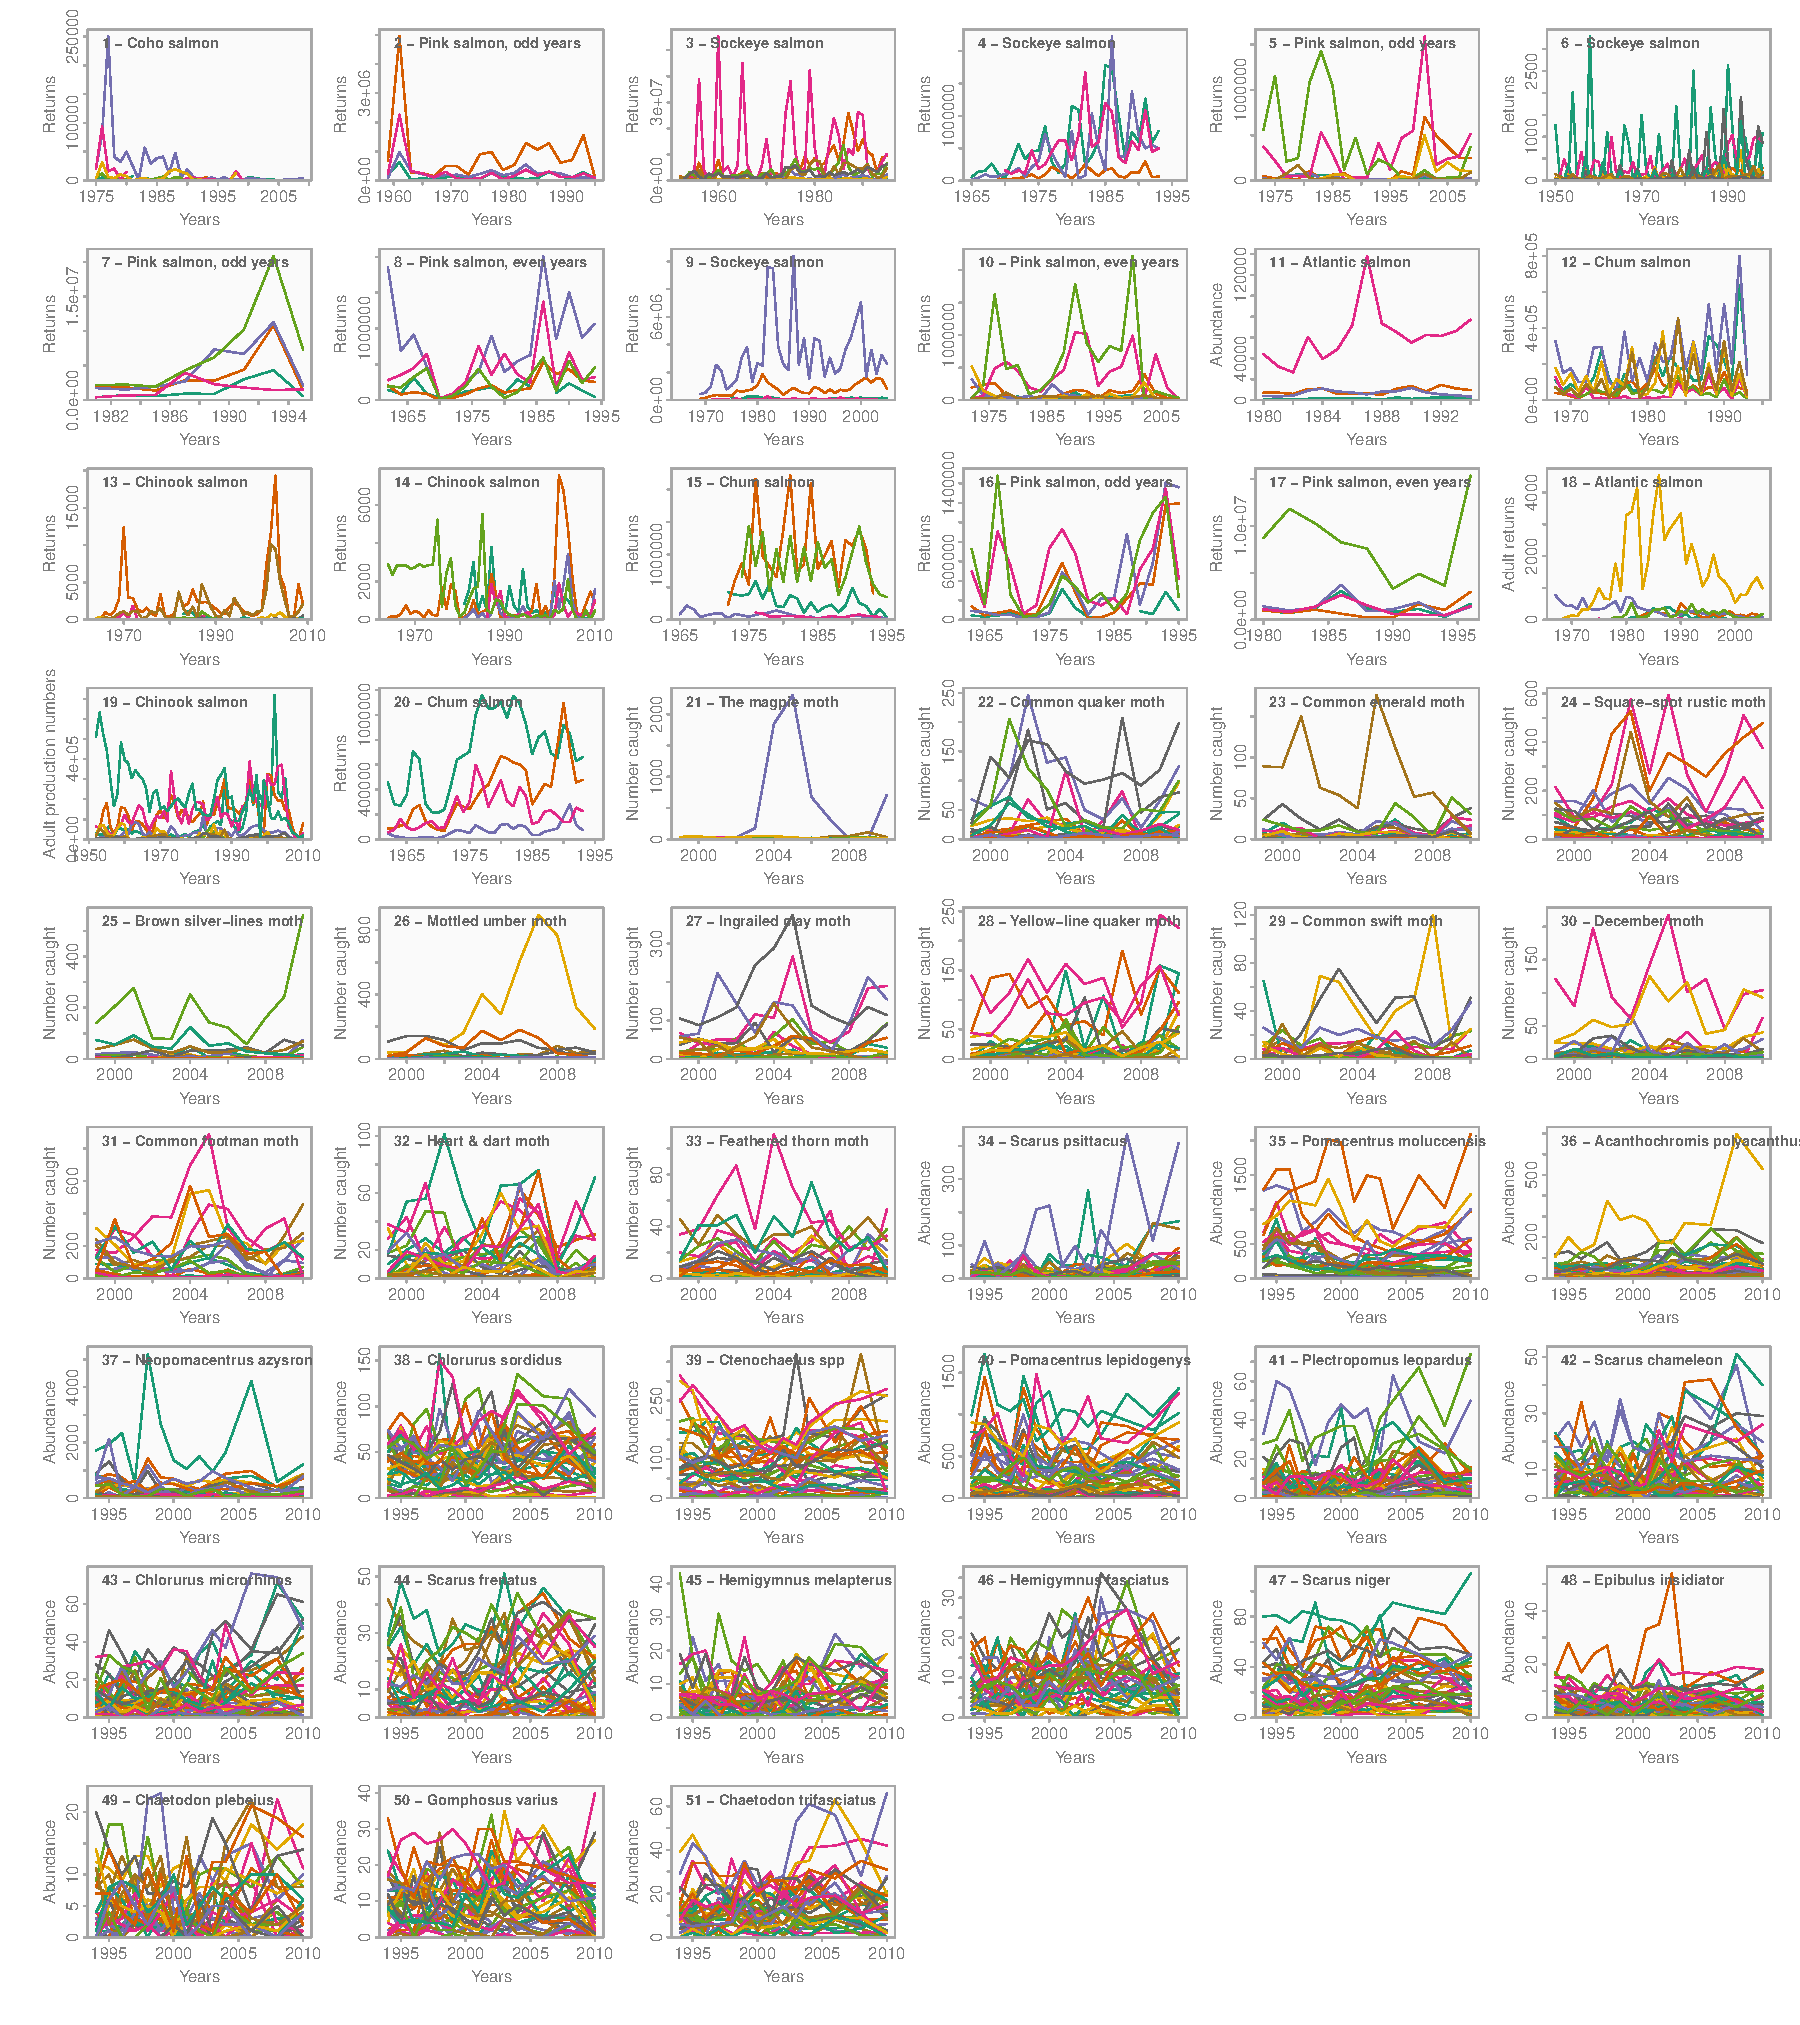
\includegraphics[width=\textwidth]{prophets/PE_data_series_ms.pdf}
  \caption[Subpopulation time series]{
    Subpopulation time series. Each panel contains one metapopulation.
    Colours were randomly assigned to distinguish subpopulations.
    Numbers in top-left corners refer to metapopulation IDs (see Table S1).
  } \label{fig:ts}
\end{figure}

\clearpage

\begin{figure}[htbp]
  \centering 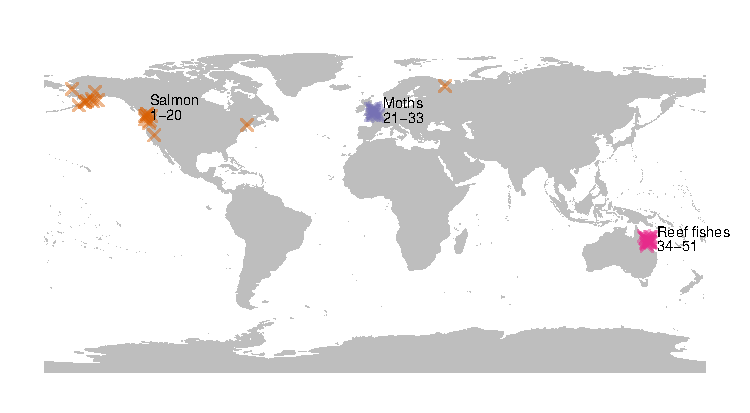
\includegraphics[width=5.5in]{prophets/PE_map_20120718.pdf}
  \caption[Map of included metapopulation]{
    Map of included metapopulations.  We represented salmon metapopulations
    with orange symbols, moths with purple, and reef fishes with pink.
    Numbers refer to metapopulation IDs (Table~S1).  Points are jittered
    slightly for visual clarity.
  }
  \label{fig:map}
\end{figure}

\begin{figure}[htbp]
  \centering
  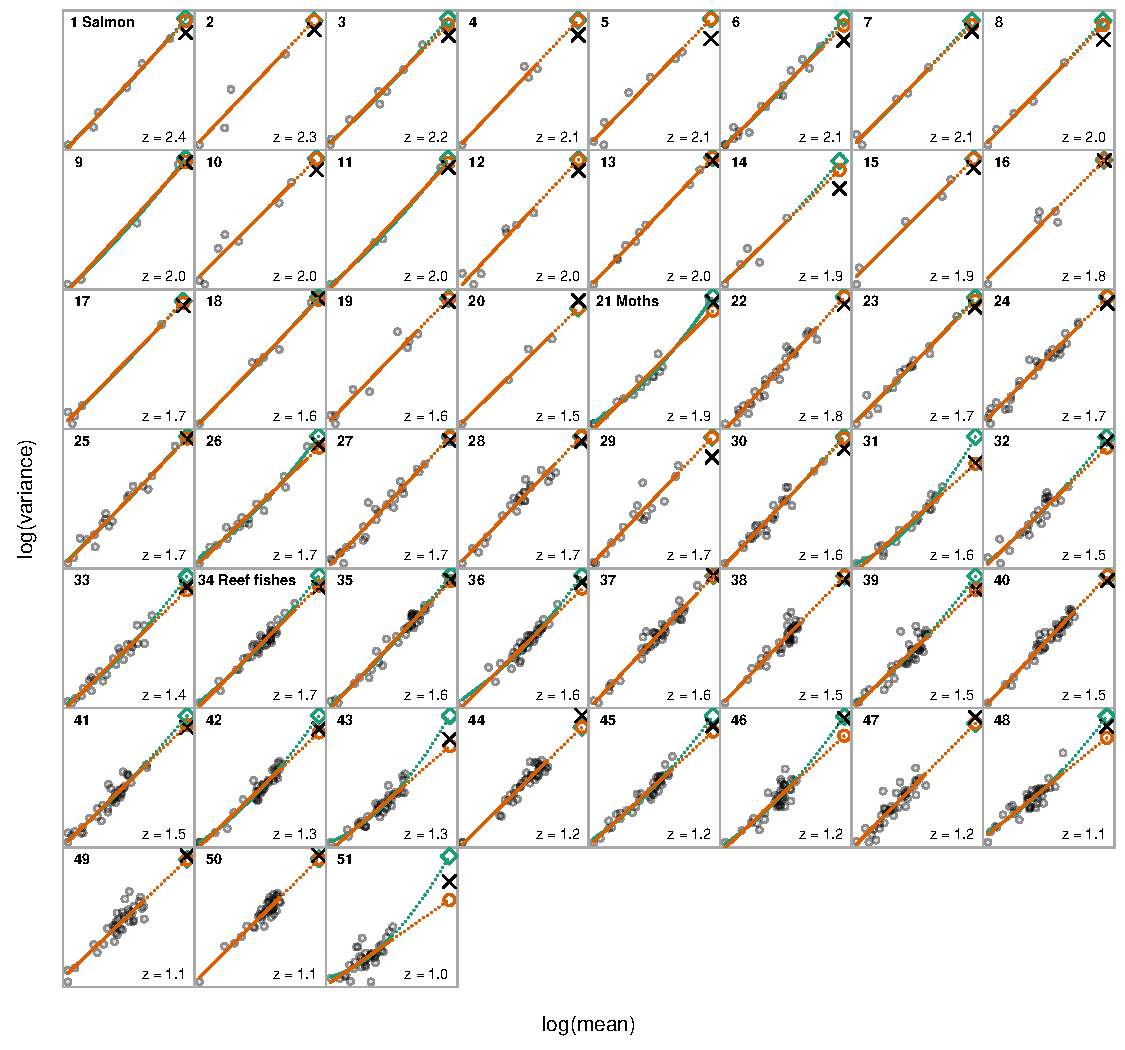
\includegraphics[width=\textwidth]{prophets/taylor-fits-scatter-20120720.pdf}
  \caption[Calculation of the \tilmanPE\ using Taylor's power law.]{Calculation of the \tilmanPE\ using Taylor's power law. Each
    dark-grey circle  represents the log($\mu$) and log($\sigma^2$) of an
    individual subpopulation timeseries.  The orange lines represent fitted
    linear regressions.  The green lines represent fitted quadratic
    regressions.  Black \texttt{x} symbols represent the observed
    metapopulation or portfolio mean and variance.  Dashed lines indicate the
    extrapolation of the model fit to the observed metapopulation or portfolio
    mean and variance.  Open-orange circles represent the predicted variance
    under the linear-fit assumption.  Open-green diamonds represent the
    predicted variance under the quadratic-fit assumption.  Metapopulations in
    which the predicted variance is greater than the observed variance
    represent variance-reducing PEs.  We ordered the panels by decreasing
    Taylor's power law \zvalue\ (slope of the linear regression) within
    taxonomic groupings.  Numbers in upper left of panels refer to
    metapopulation IDs (Supplementary Table 1)}
\label{fig:Taylor-fits}
\end{figure}

\begin{figure}[htbp]
  \centering
  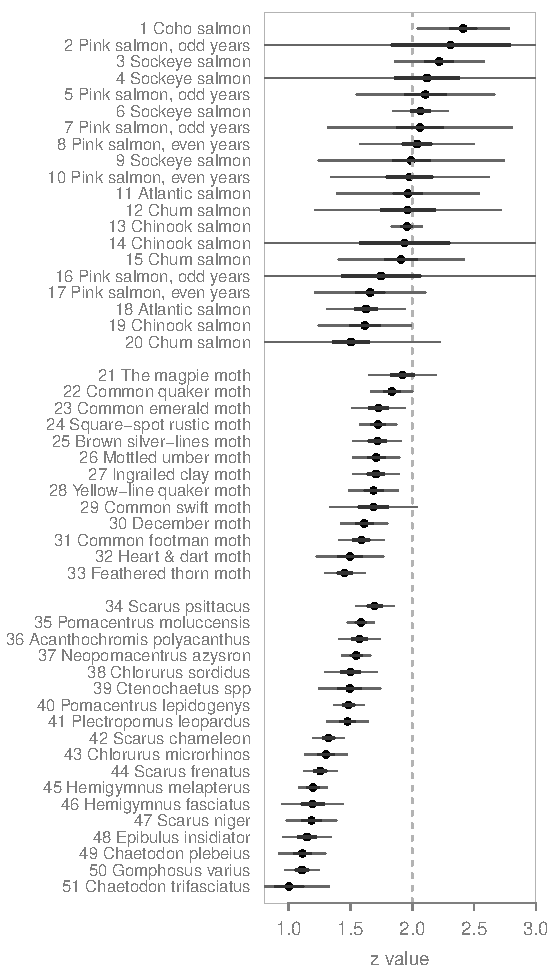
\includegraphics[height=6.6in]{prophets/Taylor_z_values.pdf}
  \caption[Taylor's power law z values across metapopulations.]{
    Taylor's power law z values across metapopulations. Points represent maximum
    likelihood estimates, thick line segments represent 50\% confidence
    intervals, and thin line segments represent 95\% confidence intervals. The
    vertical dashed line at z = 2 represents the value assumed by the average-CV
    PE method.
}
\label{fig:z-vals}
\end{figure}

\begin{figure}[htbp]
  \centering
  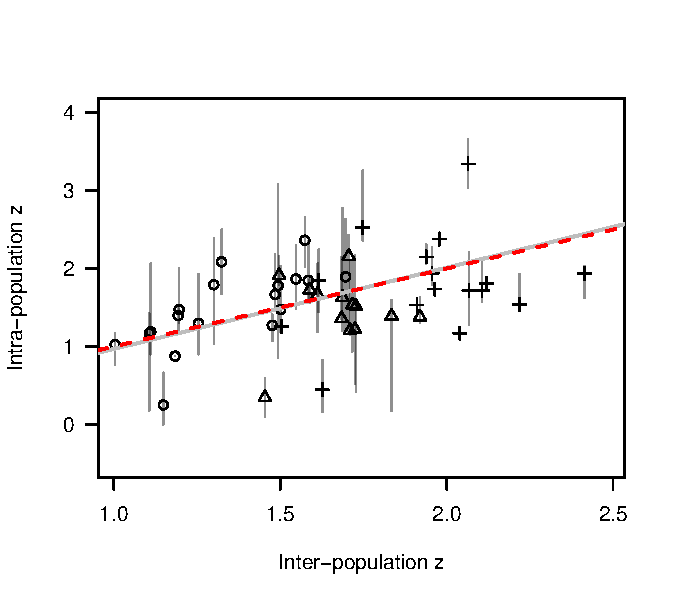
\includegraphics[width=4in]{prophets/inter-vs-intra-pop-z-seg-2-0-20121019.pdf}
  \caption[Intra- vs.\ inter-subpopulation mean-variance scaling relationship
    (Taylor's power law $z$-value).]{Intra- vs.\ inter-subpopulation mean-variance scaling relationship
    (Taylor's power law $z$-value).  Our estimation of the empirical
    mean-variance PE assumes that the inter-subpopulation $z$-value can
    approximate the intra-subpopulation $z$-value.  We use the
    inter-subpopulation $z$-value throughout our paper.  Here, we have also
    calculated the intra-subpopulation $z$-value for subpopulation time series
    in which the mean abundance in the 1\textsuperscript{st} or
    2\textsuperscript{nd} half of the time series is twice the magnitude of
    the other half.  Points represent median intra-subpopulation $z$-values
    within each metapopulation and vertical line segments represent
    1\textsuperscript{st} and 3\textsuperscript{rd} quartile values.  The
    dashed-red line represents a one-to-one relationship and the solid-grey
    line (under the one-to-one line) represents a linear regression of the
    median intra-subpopulation $z$-values with inter-subpopulation $z$-values.
    Symbols represent salmon (crosses), moths (triangles), and reef fishes
    (circles).}
  \label{fig:inter-vs-intra-z}
\end{figure}


\begin{figure}[htbp]
  \centering
  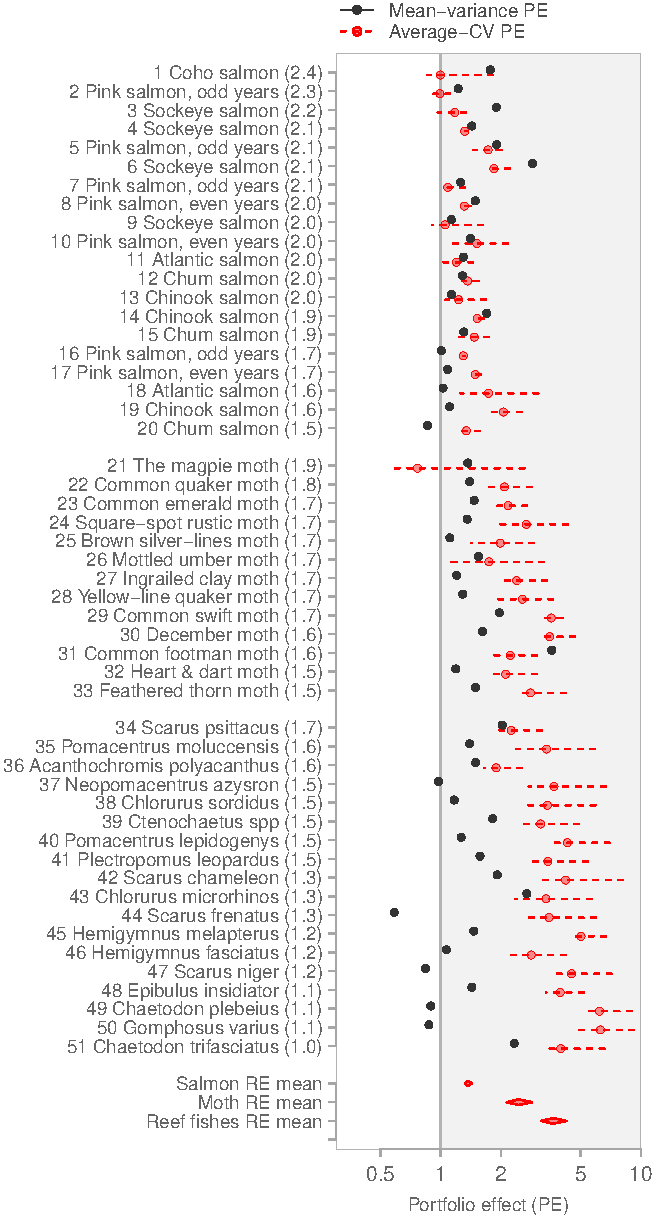
\includegraphics[height=6.8in]{prophets/PE_comparison_z_meta_taxa_quad_20121214.pdf}
  \caption[PEs with the mean-variance PEs estimated from a quadratic model.]{
    PEs with the \textbf{mean-variance PEs estimated from a quadratic model}.
    See Figure~\ref{fig:meta} for details.
}
\label{fig:meta-quad}
\end{figure}

\begin{figure}[htbp]
  \centering
  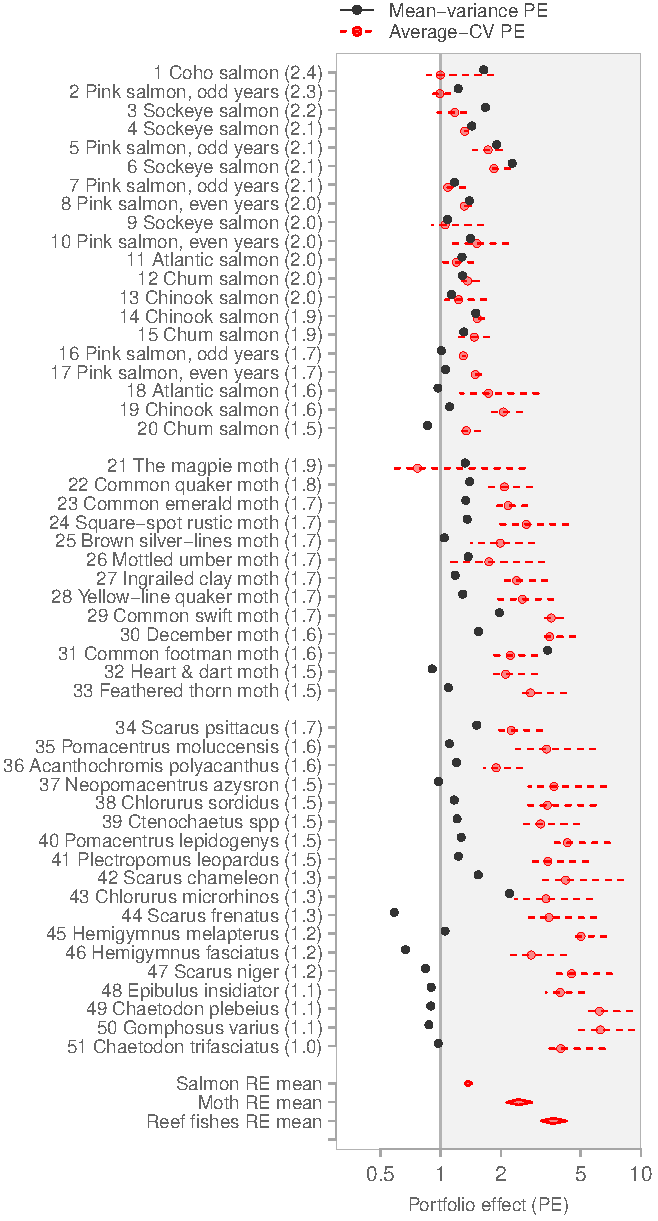
\includegraphics[height=6.8in]{prophets/PE_comparison_z_meta_taxa_lin_quad_avg_20121214.pdf}
  \caption[PEs with the mean-variance PEs estimated from a
      linear-quadratic averaged model.]{PEs with the \textbf{mean-variance PEs estimated from a
      linear-quadratic averaged model}. See Figure~\ref{fig:meta} for details.}
\label{fig:meta-lin-quad-avg}
\end{figure}

\begin{figure}[htbp]
  \centering
  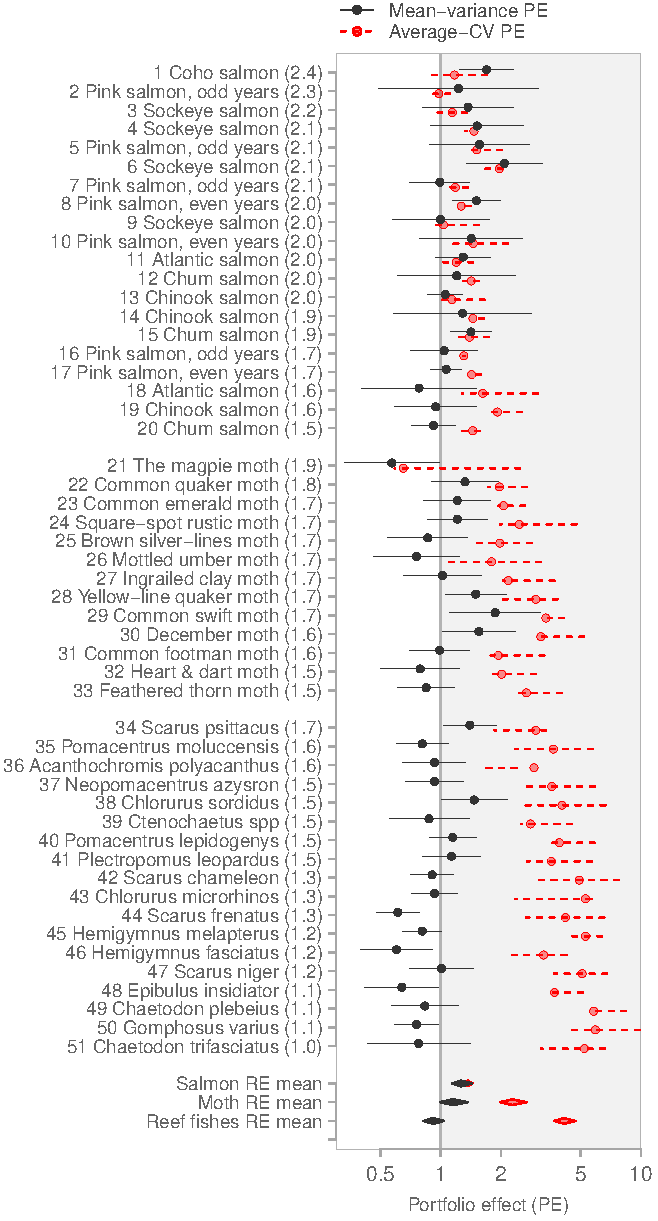
\includegraphics[height=6.8in]{prophets/PE_comparison_z_meta_detrend_taxa_20121214.pdf}
  \caption[PEs from linear detrended time series.]{PEs from \textbf{linear detrended} time series. See
    Figure~\ref{fig:meta} for details.
}
\label{fig:meta-detrend}
\end{figure}

\begin{figure}[htbp]
  \centering
  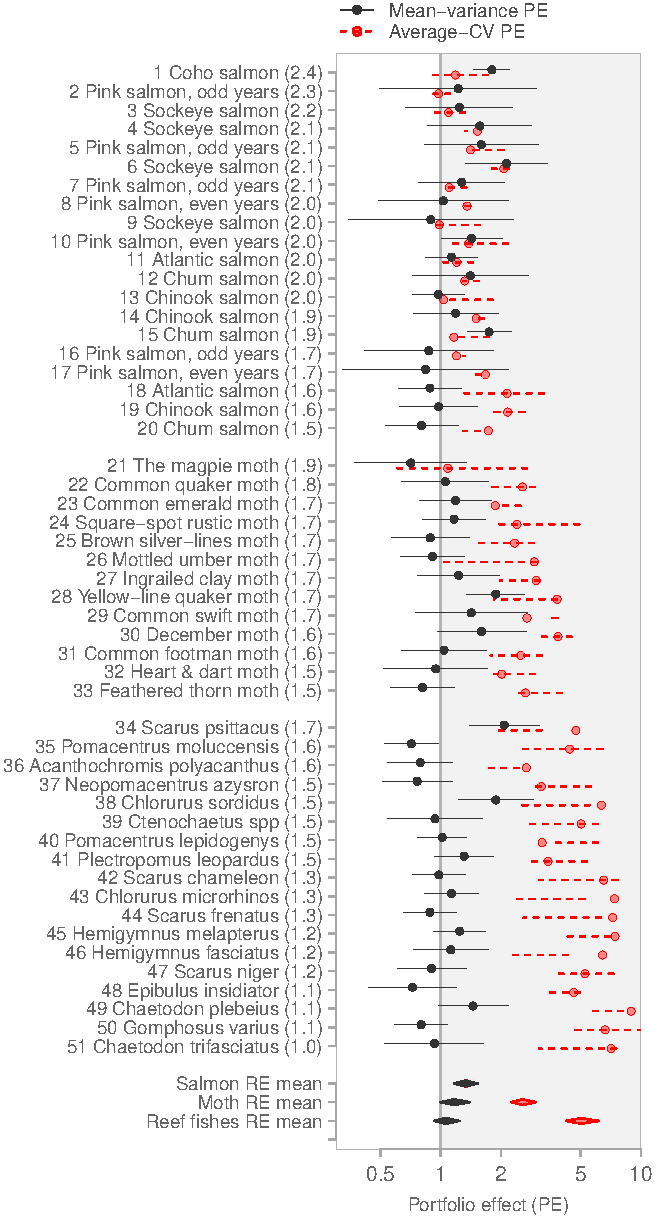
\includegraphics[height=6.8in]{prophets/PE_comparison_z_meta_loess_detrend_taxa_20121214.pdf}
  \caption[PEs from loess detrended time series]{PEs from \textbf{loess detrended} time series. See
    Figure~\ref{fig:meta} for details.
}
\label{fig:meta-detrend-loess}
\end{figure}
\clearpage

\begin{figure}[htbp]
  \centering
  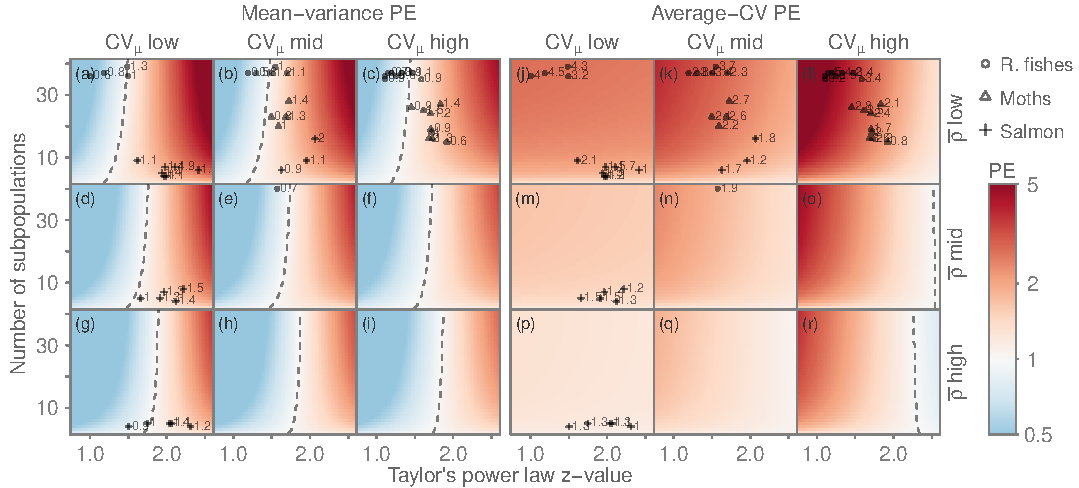
\includegraphics[width=\textwidth]{prophets/PE-parameter-space-labels-20120614.pdf}
  \caption[Empirical ecological PEs overlaid in theoretical PE
    parameter space.]{Empirical ecological PEs (points) overlaid in theoretical PE
    parameter space (colour shading). \textbf{This is the same as
    Figure~\ref{fig:paramspace} except that here we indicate the empirical PE values
      beside the points}. The colour shading indicates the
    stabilizing-effect of the theoretical mean-variance PEs (a--i) and
    average-CV PEs (j--r): red indicates a stabilizing effect and blue indicates
    a destabilizing effect.
    The dashed lines indicate neutral PEs. Columns from left to right
    show systems with increasingly uneven subpopulation sizes,
    and rows from top to bottom show systems with increasingly strong mean
    correlation between subpopulation
}
\label{fig:paramspace-labels}
\end{figure}
\clearpage

\begin{figure}[htbp]
  \centering
  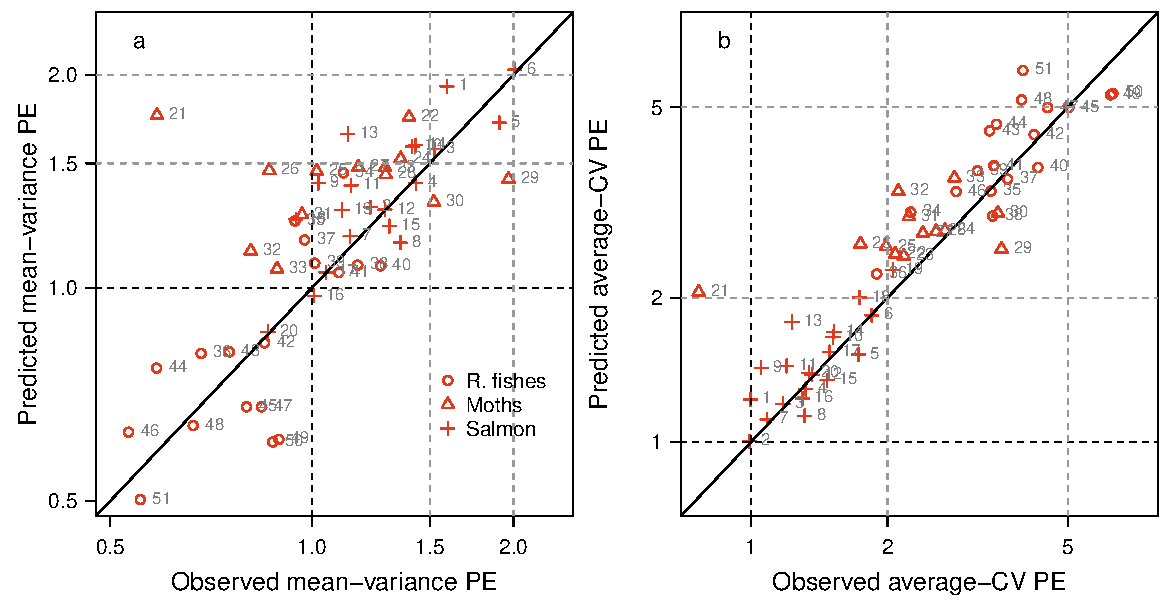
\includegraphics[width=\textwidth]{prophets/parameter-space-predicted-vs-observed-20120430.pdf}
  \caption[Predicted vs.\ observed mean-variance and average-CV
    PEs.]{ Predicted vs.\ observed mean-variance (\textbf{a}) and average-CV
    PEs (\textbf{b}).  Predicted PEs correspond to the colour underlying the
    metapopulations displayed in Figure~\ref{fig:paramspace}; observed PEs to
    the values calculated directly from the empirical data and shown in
    Figure~\ref{fig:meta}. The predicted PEs are approximate due to other
    statistical properties of the data beyond the four examined in
    Figure~\ref{fig:paramspace}, and due to grouping the $CV_{mu}$ and
    correlation values from the metapopulations to match the displayed
    theoretical values in the bins.  Numbers indicate the metapopulation IDs
    used throughout the paper (Table S1).  The solid sloped lines indicate
    one-to-one relationships.  Note that all axes have been log transformed
    and the two panels have separate axis limits.  }
  \label{fig:PE-predicted-observed}
\end{figure}

\begin{figure}[htbp]
  \centering
  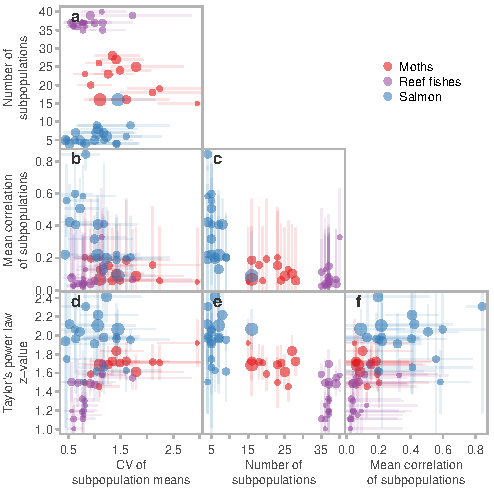
\includegraphics[height=4.6in]{prophets/bias_factors_cross_correlation.pdf}
  \caption[Relationship between the drivers of the PE in empirical systems for
    moths (red), reef fishes (purple), and salmon (blue).]{Relationship between the drivers of the PE in empirical systems for
    moths (red), reef fishes (purple), and salmon (blue).  The area of the
    filled circles corresponds to the strength of the \tilmanPE\ with larger
    circles corresponding to more stabilizing PEs.  Line segments indicate
    95\% confidence intervals.}
  \label{fig:factors-cor}
\end{figure}

\begin{figure}[htbp]
  \centering
  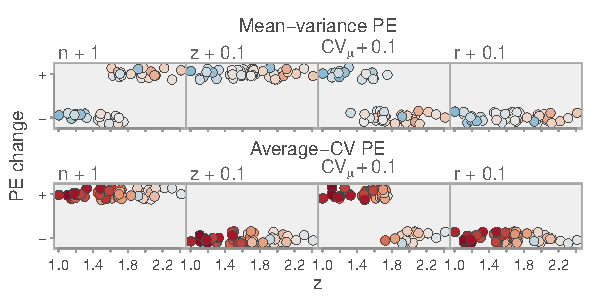
\includegraphics[width=5in]{prophets/PE-as-index.pdf}
  \caption[The PE used as an index of ecosystem change.]{ The PE used as an index of ecosystem change.  The upper panel
    shows the mean-variance PE and the lower panel the average-CV PE.  The
    horizontal axis shows Taylor's power law $z$-value.  The vertical axis
    shows the change in the PE (more stabilizing = $+$, less stabilizing =
    $-$).  The panels from left to right indicate an increase in the number of
    subpopulations ($n + 1$), Taylor's power law $z$-value ($z + 1$),
    subpopulation unevenness ($CV_{\mu} + 0.1$), or the correlation between
    subpopulations ($r + 0.1$). The quantities added are arbitrary and the
    results would look the same for any quantity added greater than zero.  Each
    dot represents an empirical metapopulation and the colour indicates the
    observed empirical PE using the same colour scale as Figs.~4~and~5. The dots
    are jittered vertically slightly for visual clarity.  }
  \label{fig:PE-as-an-index}
\end{figure}

%\end{spacing}

%\end{document}
